% 来源：固定候选 PDF，山东文科，PDF 第1页（印刷页322），Q16。
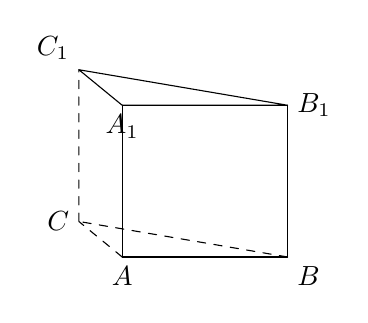
\begin{tikzpicture}[x=1cm,y=0.82cm,>=stealth,line cap=round,line join=round]
\coordinate (A) at (0,0); \coordinate (B) at (2.1,0);
\coordinate (C) at (-0.55,0.55); \coordinate (A1) at (0,2.35);
\coordinate (B1) at (2.1,2.35); \coordinate (C1) at (-0.55,2.90);
\draw (A)--(B) (A)--(A1) (B)--(B1);
\draw (A1)--(B1)--(C1)--cycle;
\draw[dashed] (A)--(C) (B)--(C) (C)--(C1);
\node[below] at (A) {$A$}; \node[below right] at (B) {$B$};
\node[left] at (C) {$C$}; \node[below] at (A1) {$A_1$};
\node[right] at (B1) {$B_1$}; \node[above left] at (C1) {$C_1$};
\end{tikzpicture}
